\section{Flask}
\subsection{Definisi Flask}
Flask merupakan micro web framework yang ditulis dalam bahasa pemrograman Python. Flask disebut micro framework karena tidak membutuhkan tools tertentu. Framework ini juga tidak mempunyai database abstraction layer, validasi form, atau komponen lainnya yang dimana sudah menyediakan library pihak ketiga yang menyediakan fungsi lain. Akan tetapi, framework flask mendukung extension yang dapat menambah fitur aplikasi seakan-akan mereka diimplementasikan dalam flask itu sendiri.
\subsection{Definis Flask Menurut Alauddin, Muhammad Fikri}
Flask adalah sebuah microframework untuk Python berbasis Werkzeug, Jinja 2 dan niat baik.Flask berfungsi sebagai pengganti PHP POST dan GET yang dimana pengendali pertukaran data dari HTML ke database. Flask juga menggantikan fungsi Apache sebagai webserver dimana flask berjalan di http://localhost:5000/.
\subsection{Instlasi Flask}
\subsubsection{On Linux}
Untuk melakukan instalasi flask, ada beberapa tahap yang harus dilakukan yaitu :
\begin{enumerate}
\item Pastikan anda sudah menginstal pyhton baik pyhton versi 2.x maupun 3.x. Jika belum instal, instal terlebih dahulu.

\item Untuk melakukan instalasi flask, kita harus membuat sebuah virtual environment lalu instal flask di dalamnya. Berikut adalah cara instal virtual enviroment / virtualenv.

\$ sudo apt-get install python-virtualenv

\item Lalu, buat satu direktori di hard disk kita untuk tempat pengerjaan project. 

\$ mkdir myproject

\$ cd myproject

\item Setelah itu, kita masuk ke direktori yang sudah di buat sebelumnya dan jalankan terminal untuk menjalankan virtualenv untuk membuat virtualenv di dalam direktori tersebut. Berikut adalah cara menjalankan virtualenv.

\$ virtualenv venv

New python executable in venv/bin/python

Installing setuptools, pip............done.

\item Lalu, berikut adalah cara untuk mengaktifkan virtualenv.

\$ . venv/bin/activate 

dan jika ingin menonaktifkannya, berikut caranya 

\$ deactivate

\item Selanjutnya, kita melakukan penginstalan flask

\$ pip install Flask
\end{enumerate}
\subsubsection{On Mac OS}
1. Instal pip terlebih dahulu menggunakan perintah :

	python get-pip.py

2. Selanjutnya instal flask dengan menggunakan perintah berikut :

	sudo pip install Flask

3. Sekarang, jalankan Simple.py untuk memastikannya berfungsi dengan menggunakan perintah berikut :

	python simple.py

Lalu, jalankan di web browser dengan perintah :

http://127.0.0.1:5000/

ketika sudah selesai, hentikan server dengan menekan kontrol-C.
\subsubsection{On Windows}

1.	Pertama, bukalah command prompt lalu ketikan perintah: pip install virtualenv

2.	Lalu, buatlah folder untuk aplikasi dengan cara mengetikan perintah: mkdir coba.
Myproject bisa diganti dengan nama lain sesuai keinginan.

3.	Setelah itu, ketikan perintah untuk masuk ke dalam folder myproject: cd coba. Lalu ketikan perintah: virtualenv flask

4.	Kemudian, ketikan perintah untuk masuk ke dalam folder myproject: cd coba. Dan ketikan perintah: virtualenv flask

5.	Kemudian, ketikan perintah untuk menginstal flask sebagai berikut:
\begin{figure}[ht]
\centerline{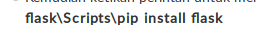
\includegraphics[scale=1]{figures/3instal.png} }

\caption{Instalasi Flask} 
\label{Flask}
\end{figure}

Pada gambar \ref{Flask} dijelaskan tentang perintah instal flask.

6.	Lalu, buat direktori app di folder mcoba dengan perintah: mkdir app

7.	Kemudian masuk ke folder app dan buat folder baru bernama: static, templates dengan perintah mkdir. Sehingga dalam folder app terdapat folder static dan template.

8.	Dan instalasi selesai.

\subsection{Perbedaan Flask}
\hspace{1cm} Flask adalah salah satu microframework yang dapat digunakan di pyhton yang di buat dengan toolkit wsgi dan jinja2. Tentunya flask itu sendiri memiliki banyak perkembangan dari versi pertama saat ia di publikasikan hingga yang terbaru. Disini saya akan menjelaskan tentang sedikit perbedaan antara flask versi 1,0 dan flask versi 0.12. Berikut adalah perbedaannya :
Berikut adalah tabel \ref{table:perbedaan} perbedaan flask.
\begin{table}[h]
\caption{Perbedaan Flask}

\centering
\begin{tabular}{ccc}
\hline
&Flask 1.0&Flask 0.12\\
\hline
Python version&tidak mendukung python versi 2.6 dan 3.3&Support Python 2.6 dan 3.3\\
\hline
Release Date&26 April 2018&21 Desember 2016\\
\hline
\end{tabular}
\label{table:perbedaan}
\end{table}

\subsection{Perbedaan Flask dengan Pyramid}
Python adalah Bahasa pemrograman yang banyak memiliki kelebihan salah satunya dapat digunakan untuk membangun aplikasi web. Disini akan menjelaskan perbedaan Antara web framework Python flask dan pyramid.
1.	Flask pertama kali dirilih pada April 2010 yang dibuat dan dimaintain oleh Armin Ronacher. Flask merupakan web framework yang sederhana namun dapat memperluas dengan berbagai pustaka tambahan yang sesuai dengan kebutuhan.
2.	Pyramid adalah web framework Python yang open source dan pertama kali dikembangkan pada Desember 2010, sebelumnya sudah ada sejak 2008 bernama repose.bfg namun dikembangkan kembali. Pyramid merupakan web framework yang penuh kesederhanaan, minimalis, dokumentasi yang terkini,cepat,reliable, dan terbuka.
\subsection{Perbedaan Flask dengan CherryPy}
Adapun perbedaan antara framework Flask dan CherryPy, adalah CherryPy dibuat dengan cara mengadaptasi cara pembuatan aplikasi Python yang berbasis objek. Dengan framework CgerryPy, programmer dapat terbiasa membuat aplikasi pyhon berbasis objek tanpa menemui kesulitan yang berarti. Sedangkan Flask, merupakan framework python yang sederhana yang disimpan dalam satu berkas .py. Library dari flask dapat diperluas sesuai kebutuhan penggunanya.
\subsection{Perbedaan Flask dengan Django}
1.	Flask memberikan kesederhanaan , fleksibilitas , dan kontrol yang halus . Ini tidak unopinionated (yang memungkinkan untuk memutuskan bagaimana kita ingin menerapkan banyak hal).\\
2.  Django menyediakan pengalaman menyeluruh : pengguna mendapatkan panel admin , database interface , ORM , dan struktur direktori untuk aplikasi dan proyek out of the box.
\subsection{Perbedaan Flask dengan Bottle}
1.	Bottle adalah framework web mikro WSGI yang cepat, sederhana dan ringan untuk Python . Ini didistribusikan sebagai modul file tunggal dan tidak memiliki dependensi selain dari Python Standard Library .\\
2.	Flask adalah salah satu microframework yang dapat digunakan di dalam bahasa pemrograman pyhton yang di buat dengan toolkit wsgi dan jinja2.

\section{Virtual Environtment}
\subsection{Definisi}
\hspace{1cm} Virtual Environment adalah sebuah salinan interpreter python yang dapat kita gunakan untuk proses instalasi paket secara pribadi tanpa mempengaruhi python global yang ada di sistem kita.

Apabila Kita menginstal Virtual Environment atau virtualenv dapat mencegah konflik paket dan konflik pada penerjemahan python system. Virtual Environment merupakan salah satu komponen sebelum melakukan instalasi Flask.
\subsubsection{Pada Python 3}
Dalam Python terdapat dua versi yakni python 2 dan python 3. begitupun instalasi sebuah virtual environment pada python 2 dan python 3 berbeda. Karena dengan python 3, virtual environment atau virtualenv mensupport native dengan paket venv pustaka standar python. Untuk menambahkan atau menginstal pustaka tersebut pada python 3 adalah sebagai berikut :

\$ sudo apt-get install python3-venv
\subsubsection{Pada Python 2}
Pada Pembahasan sebelumnya telah membahas instalasi virtual environment pada python2. Nah sekarang kami akan membahas pada python2. Pada python2 tidak terdapat pustaka venv. Oleh karena itu, virtual environment pada python 2 ini venv sebagai pustaka pihak ketiga.
Untuk menambahkan pustaka tersebut pada sistem kita adalah sebagai berikut :

\$ sudo pip install virtualenv
\subsubsection{Perbedaan Virtualenv}
Pada pembahasan sebelumnya telah membahas tentang membuat virtual environment pada python 3 dan python 2. sehingga dapat ditarik kesimpulan bahwa :
pada python 2, paket venv merupakan paket pustaka yang bersifat pustaka pihak ketiga. Sedangkan pada python 3, paket venv merupakan paket pustaka standar yang sudah disediakan oleh python.
Berikut adalah tampilan dalam bentuk tabelnya.

Berikut adalah tabelnya \ref{table:perbedaan1}.
\begin{table}[h]
\caption{Perbedaan Virtual Environment}

\centering
\begin{tabular}{ccc}
\hline
&Python 2&Python 3\\
\hline
paket venv&third party library&library standar python\\
\hline
\end{tabular}
\label{table:perbedaan1}
\end{table}


\section{Fitur Pada Flask}
\subsection{Fitur Pada Framewor Flask}
Framework flask memiliki bebrapa fitur yang dapat mendukung pembuatan web. Fitur-fitur tersebut diantaranya : 
1.	Berisi developing server dan debugger.
2.	Dukungan terintegrasi untuk pengujian.
3.	RESTful request dispatching.
4.	Menggunakan Jinja2 template engine.
5.	Dukungan untuk secure cookies (sisi klien sesi).
6.	100% WGI 1.0 compliant.
7.	Berbasis Unicode
8.	Dokumentasi yang ekstensif.
9.	Kompatibilitas Google App Engine
10.	Ekstensi yang tersedia untuk meningkatkan fitur-fitur yang dibutuhkan.

\section{Sejarah Flask}
\subsection{Sejarah Menurut Wikipedia}
Awalnyaa, Flask dibentuk dari Pocco oleh kelompok pecinta Python internasional. Pencipta flask adalah Armin Ronacher dari Pocco. Dasar dari flask adalah Werkzeurg WSGI toolkit dan Jinja2 template engine, keduanya adalah proyek-proyek Pocco yang dibuat ketika si pencipta flask dan Georg Brandi sedang membangun system papan bulletin yang ditulis dalam Bahasa pemrograman Python.

\subsection{sejarah lain}
Awalnyaa, Flask dibentuk dari Pocco oleh kelompok pecinta Python internasional. Pencipta flask adalah Armin Ronacher dari Pocco. Dasar dari flask adalah Werkzeurg WSGI toolkit dan Jinja2 template engine, keduanya adalah proyek-proyek Pocco yang dibuat ketika si pencipta flask dan Georg Brandi sedang membangun system papan bulletin yang ditulis dalam Bahasa pemrograman Python. Meskipun banyak kekurangan, Flask telah menjadi sangat populer di kalangan penggemar Python. Pada pertengahan tahun 2016. 
\subsection{install flask}
untuk menginstal flask ke dalam virtual evironment, pastikan virtual evironment venv diaktifkan, dan jalankan perintah berikut :\\
\$ pip install flask\\
ketika Anda menjalankan perintah ini, pip tidak hanya akan menginstal flask, tetapi juga semua dependensinya. Selanjutnya jalankan perintah berikut :\\
\$ pip freeze\\
dan selanjutnya import flask ke dalam python dengan perintah berikut :\\
\$ pyhton\\
import flask
\subsection{Contoh Kode Flask}
Pada kesempatan kali ini saya akan memberikan salah satu contoh kode flask, tentu banyak sekali contoh kode flask. Tetapi disini kami akan memberikan contoh kode untuk mencetak “Hello World!”. Berikut adalah contoh kodenya, semoga bermanfaat :
from flask import Flask
app = Flask(name)

@app.route("/")
def hello():
    return "Hello World!"

if name == "main":
    app.run()
\subsection{Tentang Virtualenv}
Untuk menginstall flask, alangkah baiknya menginstall Virtualenv terlebih dahulu. Virtualenv adalah alat yang berguna yang nantinya akan membuat lingkunan pengembangan Python yang terisolasi dimana user bisa mengerjakan semua pengembangan yang diperlukan. Virtualenv juga berguna untuk membuat sandbox dimana jika user menginstall seluruh library tidak akan mengganggu library lain yang pernah diinstall.
\subsection{Development web server flask}
Aplikasi flask termasuk server web pengembangan yang dapat dimulai dengan perintah jalankan flask. perintah ini dijalankan  untuk mencari nama skrip python yang berisi contoh aplikasi dalam flaskapp environment variable.
Untuk menjalankan hello.py harus menginstal virtual environment terlebih dahulu dan pastikan flask sudah terinstal. Selanjutnya jalankan perintah berikut :\\
\$ export FLASKAPP=hello.py\\
\$ flask run\\
Selanjutnya uka web browser dan masukkan perintah https://localhost:5000/ di dalam address bar.

\subsection{Mengatur Struktur Proyek}
Sebelum membuat website dengan framework flask, alangkah baiknya kita mengatur struktur proyek. Untuk mengaturnya, kita buat beberapa folder dan file di dalam flaskapp/ untuk membuat aplikasi web kita tetap rapi. Di dalam flaskapp/, buat sebuat folder app/ untuk menyimpan semua file. Di dalam app/, buat folder static/, disinilah user akan menyimpan gambar, CSS, dan file JavaScript aplikasi web. Jadi, buatlah folder untuk masing-masing jenis tersebut. Selain itu, buat juga folder bernama tempaltes/ untuk menyimpan template yang nantinya akan digunakan untuk aplikasi web. Buat juga file Python kosong bernama routes.py untuk logika aplikasi seperti routing URL.
